%    JJJ    AA     CCCCCC KKK   K TTTTTT HH  HH EEEEEE BBBBBB UU  UU SSSSSS    CCCCCC OOOOOO MM  MM
%    JJJ   AAAA    CCCCCC KKK  K  TTTTTT HH  HH EEEEEE BB   B UU  UU SSS       CCCCCC OOOOOO MM  MM
%    JJJ  AA  AA   CC     KKK K     TT   HHHHHH EEE    BB   B UU  UU SSS       CC     OO  OO MMMMMM
%    JJJ AA    AA  CC     KKKK      TT   HHHHHH EEEEEE BBBBBB UU  UU  SSSSS    CC     OO  OO M MM M
%    JJJ AAAAAAAA  CC     KKK K     TT   HH  HH EEE    BB   B UU  UU    SSS    CC     OO  OO M MM M
% JJJJJJ AA    AA  CCCCCC KKK  K    TT   HH  HH EEEEEE BB   B UUUUUU    SSS .. CCCCCC OOOOOO M MM M
% JJJJJJ AA    AA  CCCCCC KKK   K   TT   HH  HH EEEEEE BBBBBB UUUUUU SSSSSS .. CCCCCC OOOOOO M MM M
% 
% Texte Geschrieben von Stefan Bopp und Chantal Frunz
% Mehr Informationen sind auf jackthebus.com zu finden

\subsection{Tag 1}

\begin{wrapfigure}{R}{0.45\textwidth} 
  \begin{centering}
    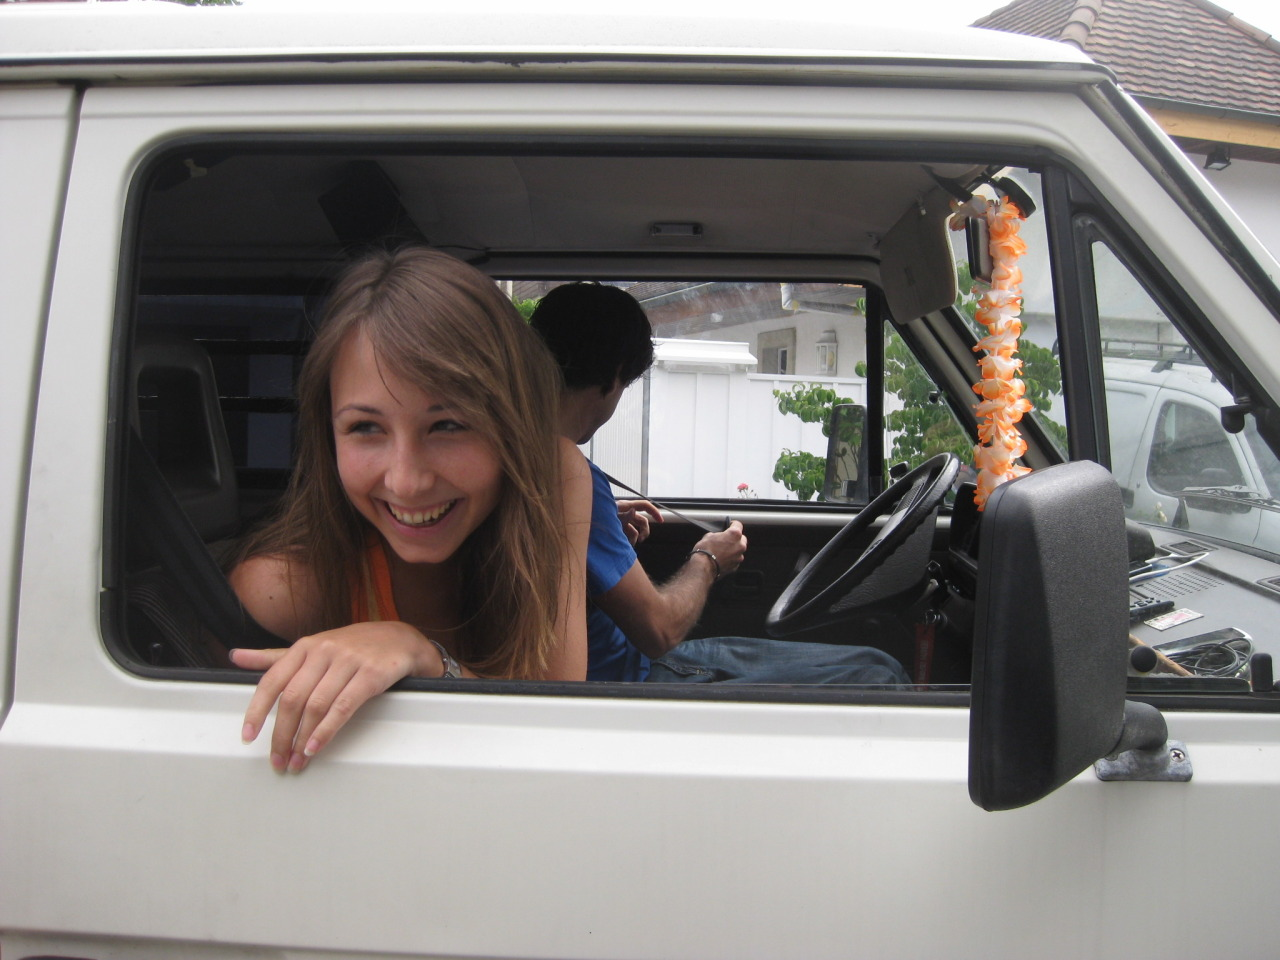
\includegraphics[width=0.4\textwidth, height=5cm, keepaspectratio]{../Bilder/Flims/2.jpg}
    \caption{Abfahrt}
  \end{centering}
\end{wrapfigure} 

\begin{figure}[b]
   \centering
      %\subfloat[CAPTION]{BILDERCODE}\qquad
   \subfloat{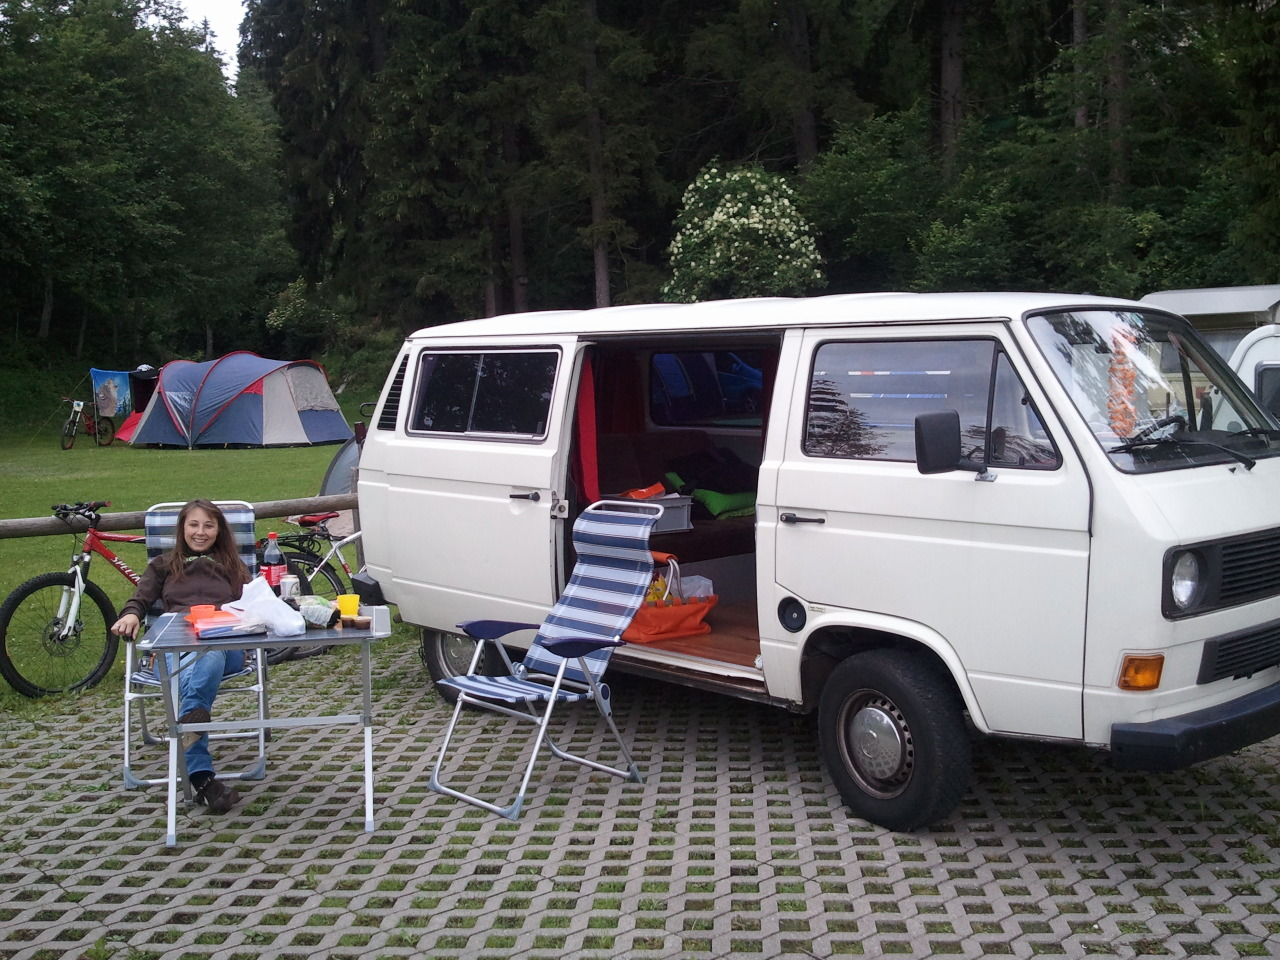
\includegraphics [width=0.3\textwidth]{../Bilder/Flims/4.jpg}}\quad
   \subfloat{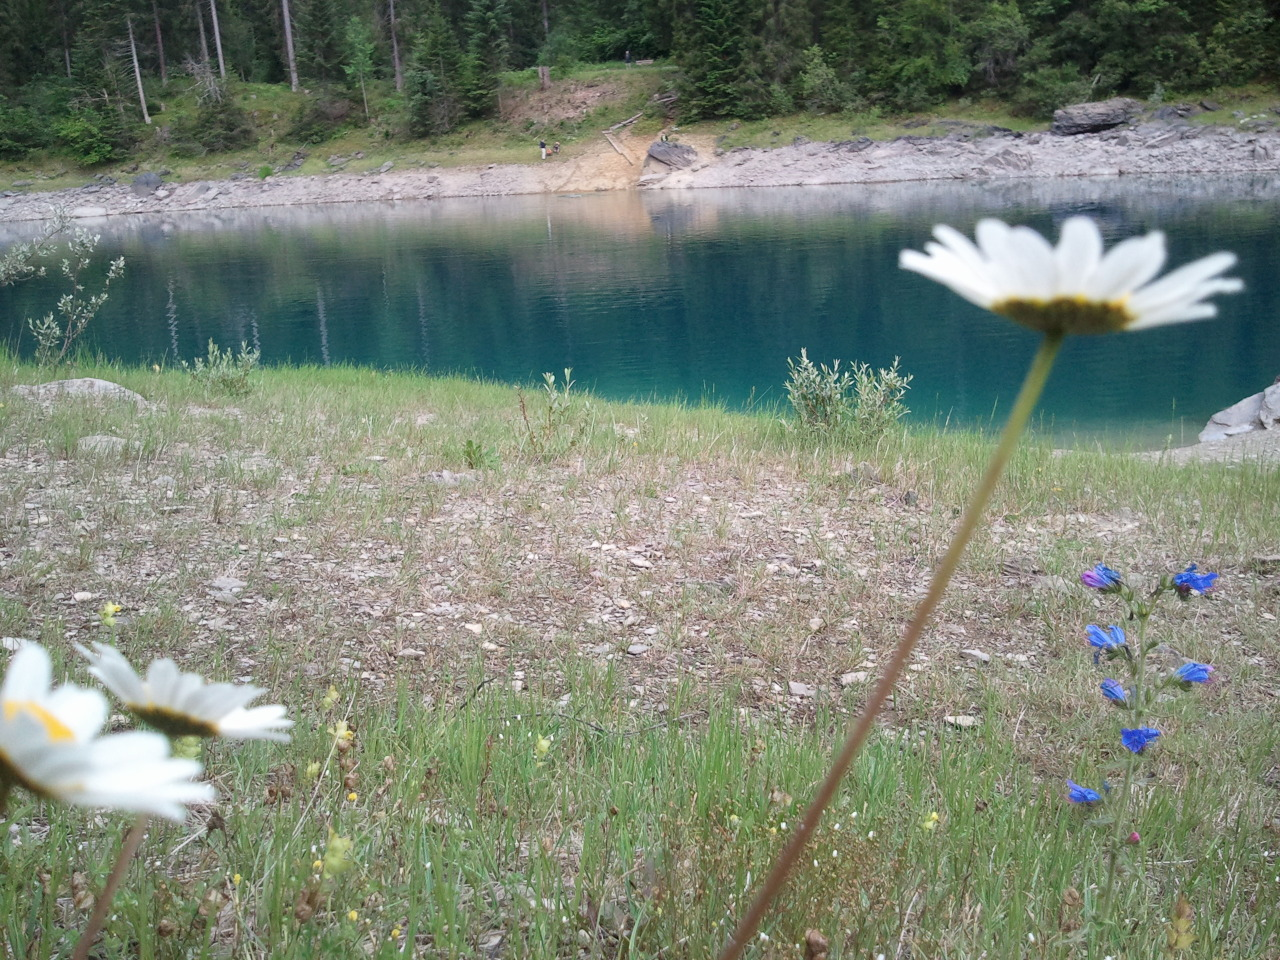
\includegraphics [width=0.3\textwidth]{../Bilder/Flims/8.jpg}}\quad
   \subfloat{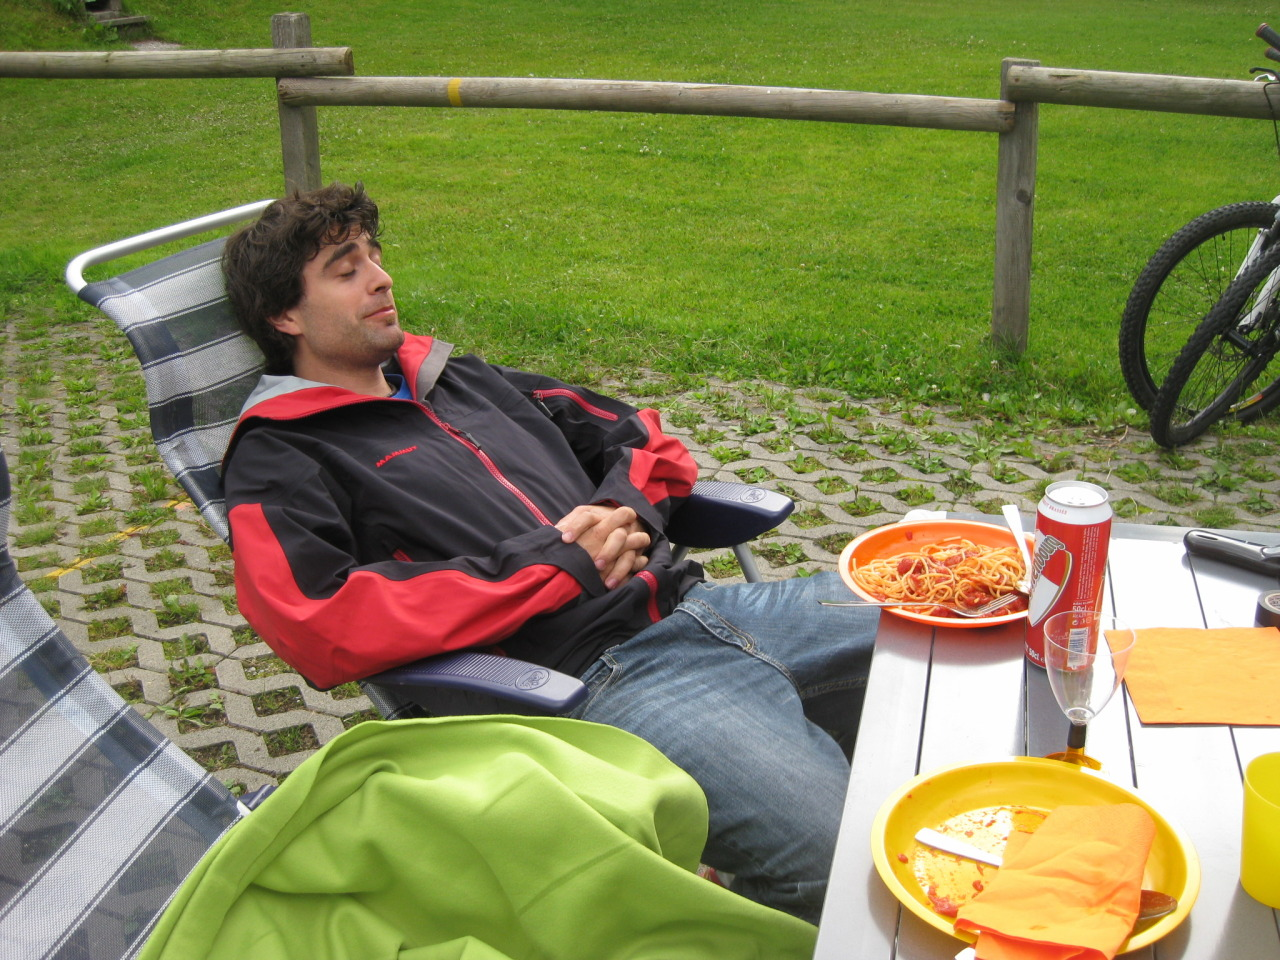
\includegraphics [width=0.3\textwidth]{../Bilder/Flims/15.jpg}}\quad
   \caption[Caumasee und Campingplatz]{Caumasee und Campingplatz}
\end{figure}

Als Geburtstagsgeschenk überraschte mich Chantal mit der frohen Nachricht, dass es am Samstag nach Flims gehen soll.
In Flims fand an diesem Weekend gerade auch noch der Trail Fox statt.
Perfekt für eine erste Probe des schon Geleisteten.
Geplant war die Abfahrt um spätestens halb 9.
Es kam jedoch anders als gedacht.
Wir brachen kurz nach 10 auf und waren um 10 nach 10 schon wieder zurück.
Meine Beifahrerin hat die falsche Schuhwahl getroffen.
Spätestens jetzt konnte uns nichts mehr aufhalten.

10 Minuten später...
Tank musste gefüllt werden.
Von nun an lief alles problemlos bis ins bekannte Heidiland.
Diesen Stopp benutzten wir um unsere Vorräte aufzufrischen und fuhren danach ohne weiteren Unterbruch auf den Campingplatz.
Leider war jedoch niemand an der Reception.
Daneben stand aber die Handynummer und so wurden wir telefonisch auf den Platz sieben gelotst.
Nun stand uns zum ersten Mal das aufstellen und bereitmachen des Buses bevor.
Stromversorgung funktionierte ohne zu murren und
auch der restliche Kram war schon jetzt in Rekordzeit aufgestellt.
Nach kurzer Verpflegung stand dem Spass in den Bäumen von Flims nichts mehr im Weg.
.. Seilpark wir kommen.
Jedoch hatte dieser am Samstag wegen dem Rennen nur bis vier Uhr offen.
Es blieb weniger als eine Stunde übrig und so beschlossen wir trotz bescheidenem Wetter den Cauma-See zu besuchen.
Nach unzähligen Fotos fing es leicht an zu Regnen.
In einer trockenen Pause radelten wir die 10 Minuten zum Campingplatz zurück.
Unterwegs sollte noch für das Abendessen eingekauft werden.
Wir trafen um 17:05 vor dem Volg ein, der natürlich um fünf Uhr schliesst.
In der modernen Zeit, in der wir leben ist es jedoch dank technischer Hilfsmittel problemlos möglich immer und überall einen der zahlreichen Tankstellenshops anzusteuern.
Sie stellen die Nahrungsmittelversorgung der zu spät kommenden sicher.
Auch in Flims gibt es solch einen Lebensretter.
Kurz per Google-Maps den Standort bestimmen und schon waren wir unterwegs Richtung Nahrung.
Eine Velotechnisch unfreundliche Autostrasse versperrte uns jedoch den Weg zum abendlichen Essensglück.
Jack war die Lösung.
Kurz alle Leitungen gekappt, die uns und Jack mit Energie versorgen und los ging die Fahrt in Schrittgeschwindigkeit durch die wahrhafte Flut von Dauercampern.
Das Loch im Auspuff macht sich in solch einer Situation sehr positiv bemerkbar: Vor den meisten voll verkleideten und eingezäunten Caravans sitzen regungslose Personen die einer schlechten Fasnachtspuppe gleichen.
Schon bei der ersten Fahrt zu unserem Platz spekulierten wir, welche von diesen Geschöpfen überhaupt noch am Leben sind.
Das leise Gluckern unseres VW Boxers unterstützt durch unregelmässige Fehlzündungen und mit sattem Bass aus dem Loch im Auspuff unterlegt, zwang diese Camper immerhin zu einem schiefen Blick, der als Lebenszeichen gedeutet werden konnte.
Die Tankstelle war dann schnell erreicht, jedoch wären doch einige Höhenmeter zu bezwingen gewesen um sie mit dem Fahrrad zu erreichen Das Kochen und der Abwasch ging Schulbuchmässig über die Bühne.
Chantal trumpfte sogar noch mit Champagner auf.
Jedoch vertrieb uns die kühle Brise schon sehr bald von unseren bequemen Stühlen.
Das Rennen am Abend wollten wir natürlich auch verfolgen.
So machten wir uns ein weiteres Mal Richtung Sportcenter, wo wir gerade noch die Aufräumarbeiten begutachten konnten.
Die Party, welche am Laufen sein sollte war auch nicht gerade der Bringer und so machten wir uns auf den Weg zurück in den Bus und genossen bis zum Einschlafen noch einen spannenden Film.

\subsection{Tag 2}
\begin{wrapfigure}{L}{0.45\textwidth} 
  \begin{centering}
    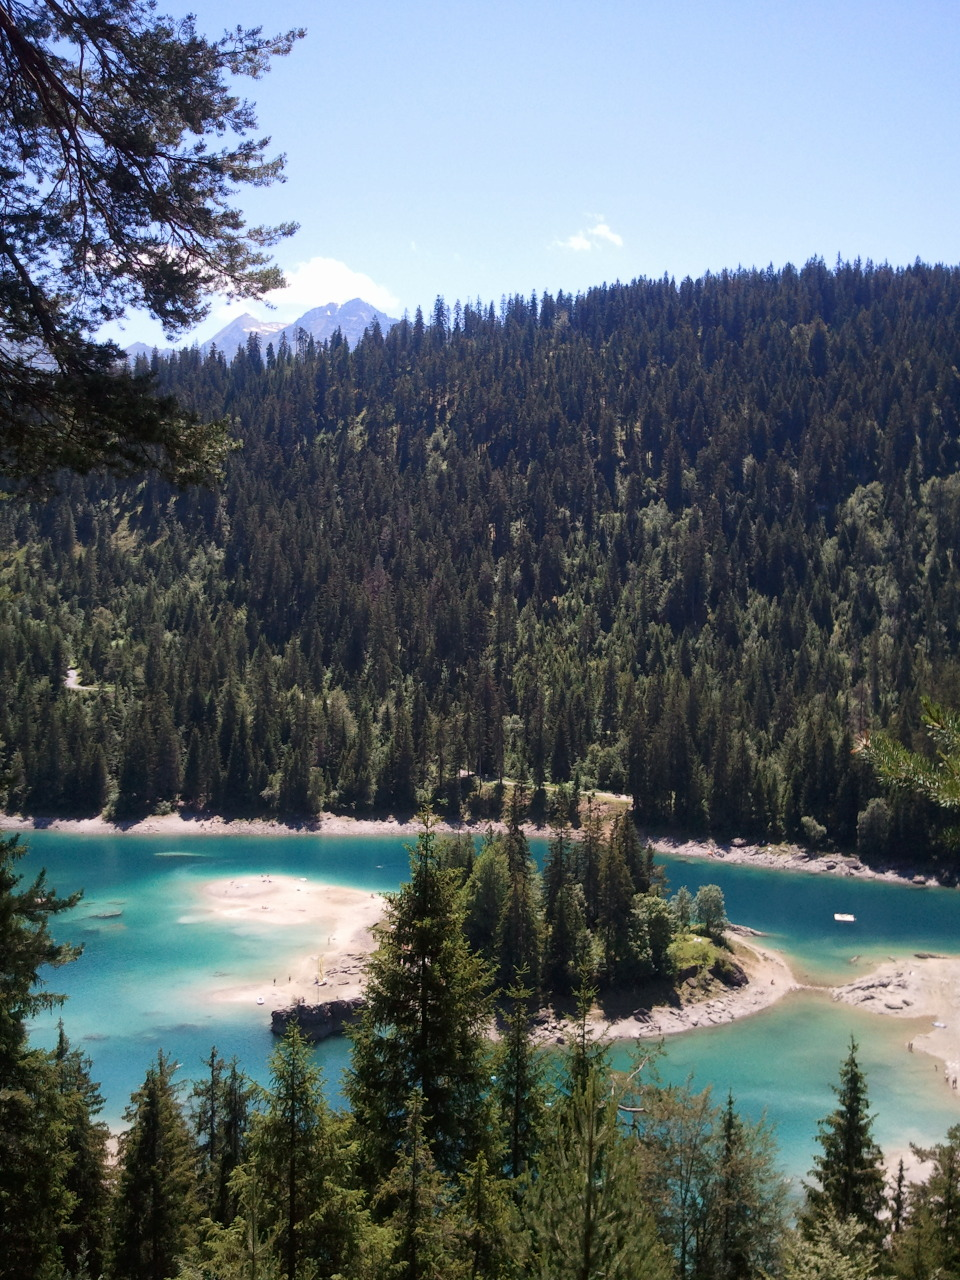
\includegraphics[width=0.4\textwidth, height=5cm, keepaspectratio]{../Bilder/Flims/21.jpg}
    \caption{Caumasee}
  \end{centering}
\end{wrapfigure} 

Nach einer kühlen aber angenehmen Nacht versuchte die Sonne durch unsere neuen Vorhänge zu scheinen und scheiterte natürlich kläglich.
Die bestellten Gipfeli waren im Laden / Reception des Campingplatzes bereit und wurden abgeholt.
Gerade als die ersten Kaffeedämpfe meine kleine Bialetti Kaffeemaschine verliessen, beschloss die Gas Buddel leer zu sein.
Kein einziger Tropfen fand den Weg nach oben durch das Kaffeepulver.
Auf an den Caumasee und die Wärme geniessen.
Meine anfänglich sehr optimistische Ankündigung zur Insel hinaus zu schwimmen wurde durch den ersten Kontakt mit dem 18°C (warmen) Wasser korrigiert.
Chantal stürzte sich natürlich todesmutig in die eisigen Fluten und schien es sogar zu geniessen.
Mit roter Nase und verbrannten Füssen machten wir uns mit den Bikes wieder an den beschwerlichen Aufstieg, damit wir dieses eine Mal auch sicher nicht zu spät sind um uns das Rennen anzuschauen.
Doch auch dieses Mal blieb uns der Erfolg vergönnt und wir sahen einmal mehr nur noch die letzten Streckenposten, die das Material zurück zum Sportcenter brachten.
Da wir schon einen Grossteil aufgeräumt hatten und so noch etwas Zeit hatten, beschlossen wir einen unbedeutenden Umweg zu machen, um noch ein paar Blicke in die Rheinschlucht zu erhaschen.
Diese konnte sich ja schlecht aus dem Staub machen.
Google Maps, zeigte sich wieder einmal von seiner schönsten Seite und Lotste uns über Wege, die normalerweise eher als Pfade bezeichnet werden würden.
Unser tapferer Bus quälte sich problemlos durch den Staub und den schier unpassierbare Gegenverkehr.
Schlussendlich wurden wir jedoch mit wunderschönen Aus und Einblicken in die Rheinschlucht belohnt.
Den Weg zurück nach Dättwil verlief ziemlich Ereignislos und mit nur geringem Stau.

\subsection{Rückfahrt}
Nach zwei wunderschönen Tagen waren wir zurück mit vielen wunderschönen Eindrücken und Erlebnisse.
Unser Ausbau hat sich grösstenteils bewährt und wir wissen nun, dass wir auf jedenfalls auf dem richtigen Weg sind.

Die Gegend um Flims haben wir sicher nichtcaumaseedas letzte Mal besucht und auch der kleine aber feine Campingplatz bleibt uns in bester Erinnerung.

\begin{figure}[hb]
    \centering
    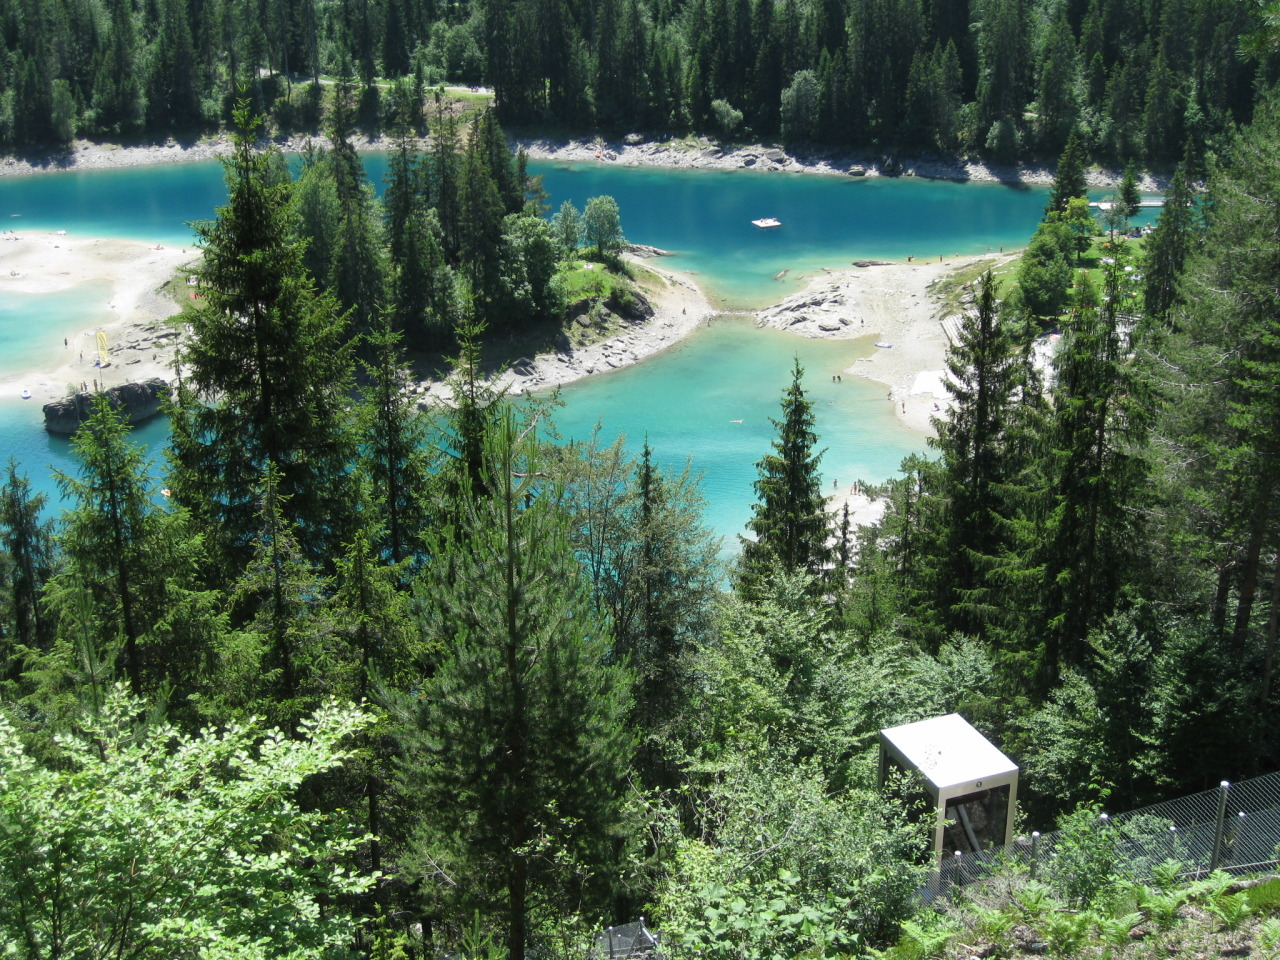
\includegraphics[width=\textwidth]{../Bilder/Flims/22.jpg}
    \caption{Caumasee}
    \label{img:Flims1}
\end{figure}
